% Chapter Template

\chapter{3D Models in Dentistry} % Main chapter title

\label{Chapter6} % Change X to a consecutive number; for referencing this chapter elsewhere, use \ref{ChapterX}

 %----------------------------------------------------
 
 
We discussed how to get a 3D digital model from diagnostic images and how to convert it into a physical model using 3D printing. Both the digital model and the physical model are elements that can elevate the quality of the therapies provided by the doctors, and at the same time those are of great value for the clinical researcher, thanks to the retrievable amount of data.\\
The fields of application are many and embrace the surgical disciplines, education and dental procedures such as implantology, prosthetics and conservative dentistry \parencite{Reference103}.
We will discuss some of the most relevant implementations of the procedures we have described.

\section{Education}
\begin{wrapfigure} {R} {0.4\textwidth}
\vspace{-20pt}
	\begin{center}
	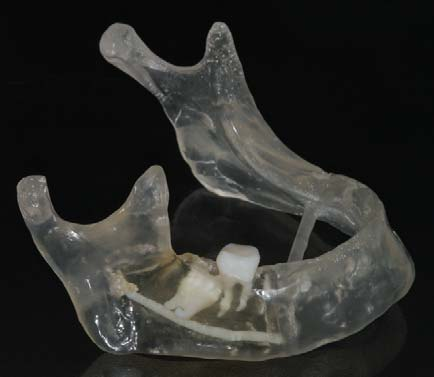
\includegraphics[width=0.4\textwidth, height=\textheight,keepaspectratio]{mandi_molar}
    \caption{Printed 3D model obtained from a CBCT. It shows the third and second molar and the inferior alveolar nerve. From \emph{Lambrecht et al} \parencite{Reference69}}
    \label{fig:mandi_molar}
    \end{center}
\vspace{-20pt}
\end{wrapfigure}
The training path of the dentist and medical doctor is a combination of theoretical lessons and practical activities, aimed at providing in-depth medical knowledge and a method of clinical reasoning. The student has to develop manual skills to perform interventions on the patient. In addition, every student in the medical field studies the \emph{human anatomy}, and if once cadavers dissection were what provided the students with a practical learning context, now few institutes offer this possibility \parencite{Reference67}. \\
With the decrease in the use of cadavers, the use of plastic replicas of parts of the body has increased as a practical complement to the learning of anatomy. Several authors have recently begun to explore the possibilities offered by modern medical modeling and 3D printing techniques in the field of medical training. \\ Anatomical models for the study of anatomy and for the explanation of operative procedures have been produced both in the medical and dental field \parencite{Reference66 }, \parencite{Reference70}. Heng \parencite{Reference67} evaluated the short-term improvement in an anatomical knowledge test for students, where 3D printed heart models and real cadaver hearts were used. He found a positive outcome in evaluating the experience with 3D models. Lambrecht \parencite{Reference69} produced models for oral surgery training by means of a stereolithographic printer (SLA), to facilitate students to learn complex surgical procedures \ref{fig: mandi_molar}.
\begin{figure}[h]
\vspace{-10pt}
	\begin{center}
	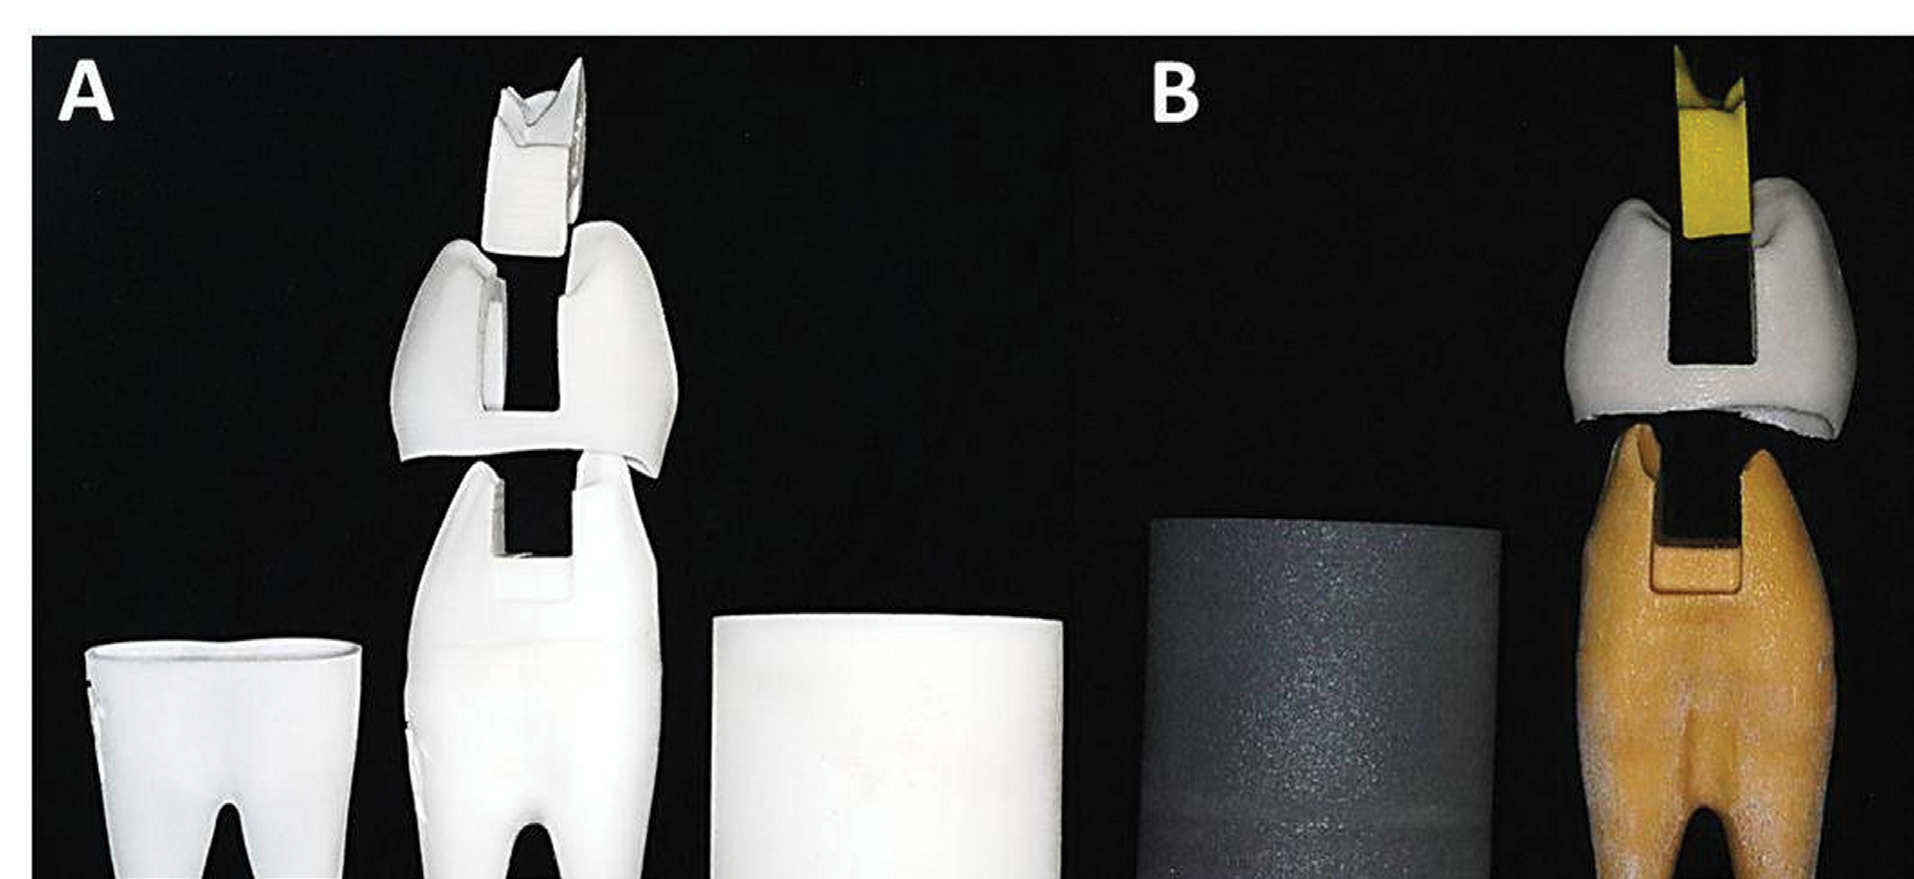
\includegraphics[width=0.8\textwidth, height=\textheight,keepaspectratio]{cavity_prep}
    \caption{Models representing cavity preparation geometry. From \emph{Soares et al} \parencite{Reference71}}
    \label{fig:cavity_prep}
    \end{center}
\vspace{-20pt}
\end{figure}
 
Soares et al \parencite{Reference71} produced models of teeth to instruct students on cavity preparation techniques \ref{fig: cavity_prep}. Other authors realized 3D models as practical support for preclinical courses, for example Kroger et al \parencite{Reference72} created models to train on caries removals and provisional prosthesis; Reymus et al \parencite{Reference73} printed replicas of teeth with endodontic cavities to simulate endodontic preparation. The common outcome of these studies was the overall positive evaluation of the 3D printed models by both the students and the teachers. 3D printers are also welcomed by students and university staff, as documented by Walker \parencite{Reference74}. \\
There are already several online libraries in which anatomical models can be found, such as the one provided by the \emph{NIH} \parencite{Reference75} and the one on the website \emph{Embodi3d} \parencite{Reference76}. Moreover, the possibilities offered by the described workflow allow to create original anatomical models of complex cases or special procedures at reduced cost. The initial effort in software learning is offset by the range of possibilities offered by the workflow in question as an aid to dentistry training.

\section{Planning of surgical intervention}
Surgical planning is an important step in the patient's treatment, because it provides the surgical team with an in-depth knowledge of the case under examination and allows to evaluate the best approach to accomplish the surgery. The digital imaging techniques (NMR, CBCT etc\ldots) associated with 3D models have been experimented by several authors with the aim of providing the surgeon with a real reference to plan the intervention. \\ Models that replicate the anatomy of the region to be operated have been created for different surgeries, from vascular surgery to orthopedic surgery. The \emph{Medical Modeling} book by Bibbs et al \parencite{Reference1} collects a series of interesting clinical, surgical, dental and research cases that show the use of medical modeling and rapid prototyping techniques. The surgeon can simulate on the models the execution of the osteotomies, simulate the new arrangement of the bone segments and create surgical guides as an aid to the surgery \parencite{Reference77}, \parencite{Reference78}.
\begin{figure}[h]
\vspace{-10pt}
	\begin{center}
	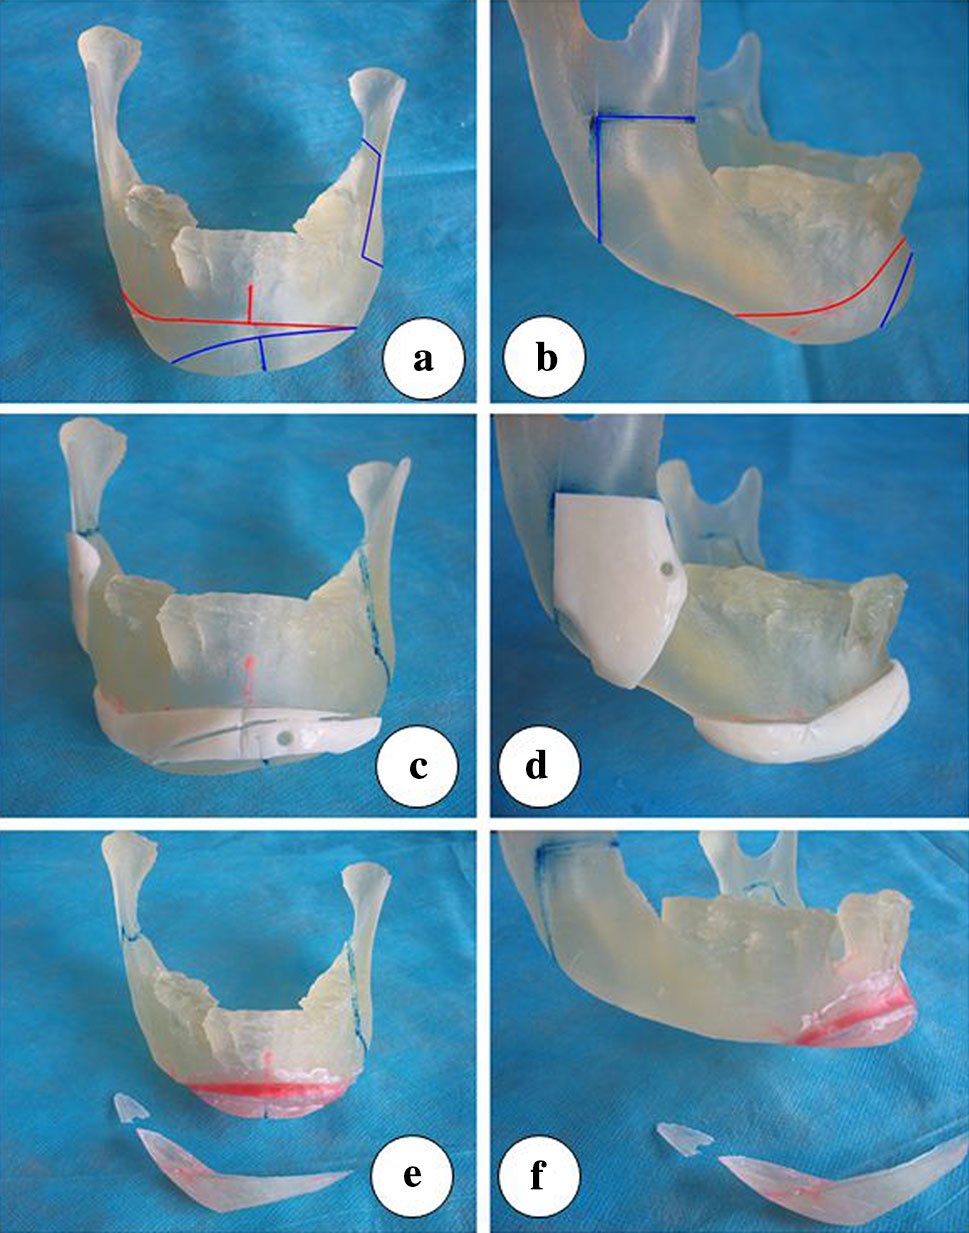
\includegraphics[width=0.5\textwidth,height=\textheight,keepaspectratio]{train_model}
    \caption{3D printed model for surgical planning.
\textbf{a}: Landmark and osteotomy lines on the 3D model (front view).\textbf{b}: side view. \textbf{c}: Surgical template (frontal view). \textbf{d}: side view. \textbf{e}: Surgery simulation (frontal view). \textbf{f}: side view. From \emph{Wang et al} \parencite{Reference20}.}
    \label{fig:train_model}
    \end{center}
\vspace{-20pt}
\end{figure}

Wang \parencite{Reference109} reported the use of 3D models to plan mandibular orthognathic surgery and for surgical guides manufacturing, noting greater speed and precision in the execution of the osteotomy and positioning of the bone segments \ref{fig:train_model}. \\
The Blender \emph{OrtogOnBlender} plugin \parencite{Reference64}, \parencite{Reference79} helps the planning of \emph{orthognathic surgery} \ref{fig:ortogon1}, facilitating the simulation of osteotomies and allowing to evaluate the consequences of bone mobilization on the patient's face. The patient's face can be scanned or detected with a series of photographs; OrtogOnBlender allows you to derive 3D models through photogrammetry, and to use these models in combination with the CT scans, enabling the use of combined models of the surface and inner part of the organism. In this way it is possible to simulate the consequences of the bone segments positioning on the patient's face  \parencite{Reference145}.

\begin{figure}[h]
\vspace{-10pt}
	\begin{center}
	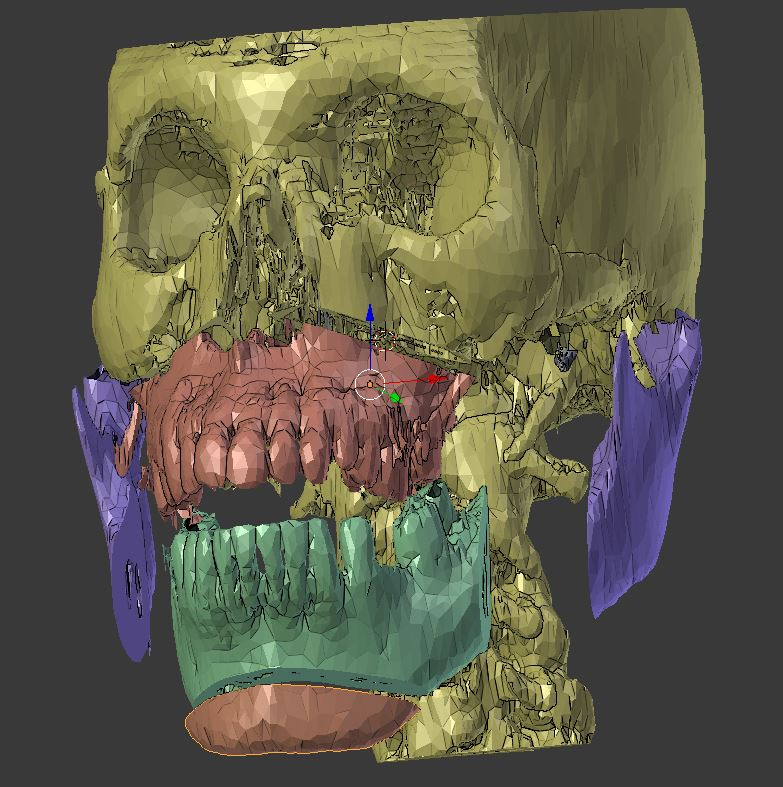
\includegraphics[width=0.6\textwidth,height=\textheight,keepaspectratio]{ortogon1}
    \caption{Virtual osteotomies made with the add-on \emph{OrthogOnBlender}}
    \label{fig:ortogon1}
    \end{center}
\vspace{-20pt}
\end{figure}


Orthognathic surgery simulation with OrtogOnBlender \parencite{Reference80} starts loading DICOM images into Blender, but an already processed .stl model can also be used. The plugin facilitates the digital osteotomies by creating cutting planes to be placed in the desired position. After the digital osteotomies we can isolate the segments and move them in the planned position. \\
The management of the pictures for the photogrammetry reconstruction is fast: after importing the folder containing the pictures, the software automatically creates the model of the patient's face. Through a few operations the scan of the face is aligned with the CT, enabling the preview of the planned surgery of the jaws.\\
Rapid prototyping technologies have been used successfully for the realization of a custom surgical obturator following the removal of an upper maxillary carcinoma \parencite{Reference81}. \\
Ackland et al \parencite{Reference82} rehabilitated a patient with \emph{Temporo Mandibular Joint} osteoarthritis (TMJ) by designing a customized prosthesis, on which they performed Finite Element Analisys (FEA) to optimize their position and fixation. The digital model was then printed in Titanium 6Al4V with an SLS printer and implanted on the patient with good results. \\
The integration of digital techniques and 3D printing in the surgical workflow can be of considerable help to the surgeon for the surgery planning, especially in cases of complex surgeries and in sensitive areas of the organism (for example, near neurovascular bundles). These technologies allow to customize any rehabilitation devices, such as prostheses that adapt to the patient's anatomy and biomechanics. Multidisciplinary collaboration in surgical planning is a building block of this rehabilitative approach focused on customization.


\section{Digital dentistry and 3D printing}

\subsection{Surgical Implant Guides}
Digital imaging is fundamental in implantology for bone evaluation and implant site selection, while modeling and rapid prototyping techniques allow to quickly create customized surgical guides, which can be sterilized and used for the insertion of the implants \parencite{Reference83}. As shown by literature analysis, the surgical guide allows to operate with greater precision than the manual insertion procedures. Van Assche \parencite{Reference105} carried out a literature review, giving indications on the use of surgical guides in implantology. The position of the implant inserted with the guides is more predictable than the manual insertion, and the guide in the implant insertion phase has a higher precision than the guidance of the sole osteotomies, where only the site preparation is guided, while the subsequent insertion of the fixture is manual. The average error found with the guides is about 1mm in the entry position, 1.3mm at the apex with an inclination difference of about 4 degrees, although with a wide variability between the analyzed studies.

\begin{figure}[h!]
 
\begin{subfigure}{0.5\textwidth}
\centering
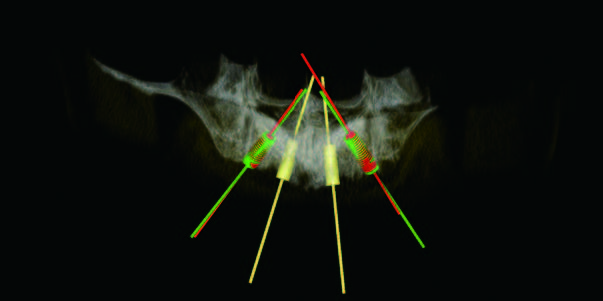
\includegraphics[width=0.9\linewidth, keepaspectratio]{beretta_digital} 
%\caption{Skirt}
\label{fig:beretta_digital}
\end{subfigure}
\begin{subfigure}{0.5\textwidth}
\centering
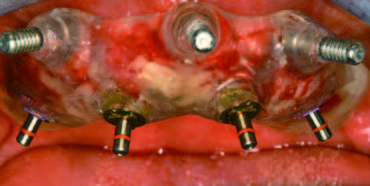
\includegraphics[width=0.9\linewidth, keepaspectratio]{beretta_real}
%\caption{}
\label{fig:beretta_real}
\end{subfigure}

\caption{\textbf{Left}: Implant planning simulation superimposed on a CT scan (red) and postoperative scan with inserted implants (green). \textbf{Right}: Surgical guide for the upper jaw, stabilized by mini-implants. From \emph{Beretta et al} \parencite{Reference104}.}
\label{fig:Beretta}
\end{figure}

Beretta \parencite{Reference104} has found similar data in the literature, but in his small series of 14 implant rehabilitations performed with surgical guides, he found lower errors. The greatest precision is attributed to some measures, such as the use of extraoral references for correct anatomical positioning, the combined use of CT scans and optical scans in positioning procedures, and intraoral fixation of the guide with mini implants \ref{fig:Beretta}. \\
According to the analyzed reports the use of the surgical guides is a valid aid to the implant insertion procedures, keeping in mind an adequate margin of error of at least 2mm from sensitive areas \parencite{Reference104}. The accuracy in the production of the guides is important, so we must try to reduce the error accumulated between the scan of the arches, the design and manufacture of the guide.
 
\subsection{Root Analog Implants}
In the field of implantology, the authors described anatomical shaped implants to be inserted in post-extraction alveolus (Root Analog Implant - RAI). These implants are made with CAD / CAM techniques of additive or subtractive manufacturing (milling), and replicate the morphology of the dental element to be replaced. The anatomy of the alveolus can be obtained through the use of a CBCT scan or with the optical scan of the extracted tooth root. The optical scan requires operating in two steps, the dentist needs to extract the tooth to scan it, create the digital model, print the implant and reopen the surgical site to insert it. The preoperative CBCT allows to plan the intervention, to create the personalized implant and then to insert it immediately after the extraction of the tooth, in a single session.
\begin{figure}[h]
\vspace{-10pt}
	\begin{center}
	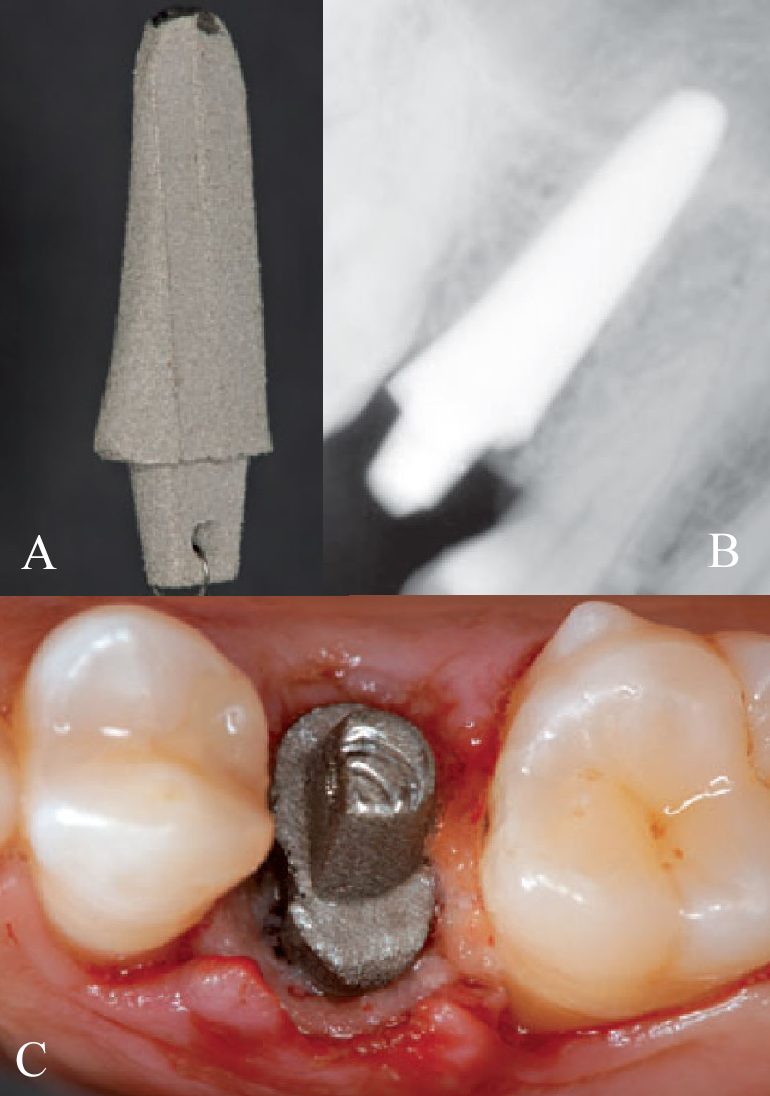
\includegraphics[width=0.5\textwidth,height=\textheight,keepaspectratio]{mangano_implant}
    \caption{DLMF Root Analog Implant. \textbf{A}: Titanium RAI. \textbf{B}: RAI in the alveolus. \textbf{C}: intraoral view of the RAI. From \emph{Mangano et al} \parencite{Reference84}}
    \label{fig:mangano_implant}
    \end{center}
\vspace{-20pt}
\end{figure}

Mangano \parencite{Reference84} used CBCT reconstructions to make the customized implants by means of DLMF (\emph{Direct Laser Metal Forming}) printing technology, which uses a laser to sinter titanium particle at layers height of 0.2 mm \ref{fig:mangano_implant}. Final ceramic crown was inserted on the RAI and the maintenance of peri-implant tissues was noted at the annual inspection.
Mangano \parencite{Reference85} then performed a study of 15 patients, using root analog implants. Although further studies are needed, the work showed how RAI made with DLMS (\emph{Direct Laser Metal Sintering}) can be a treatment option for post-extractive rehabilitation cases of dental elements where atraumatic avulsion is possible, so to keep intact corticals. \\
Pirker \parencite{Reference86} modified the root of the extracted tooth with the addition of composite macro-retentions on the distal and proximal portion, leaving the vestibular surface and the lingual surface of the root unaltered. The root thus modified was scanned with an optical scanner, and the obtained digital model was slightly reduced in the diameter of the vestibular and lingual regions (between 0.1 and 0.3 mm) to limit the risk of fracture of the alveolar corticals. The implant was then produced in zirconia using a CAD-CAM milling machine and implanted in the alveolus \ref{fig:bioimplant}. Primary stability was optimal, thanks to the use of interdental macroretention. At the 2 year follow-up there were no signs of bone resorption or gingival retraction, sign of a correct distribution of stress on the alveolus wall.
\begin{figure}[h]
\vspace{-10pt}
	\begin{center}
	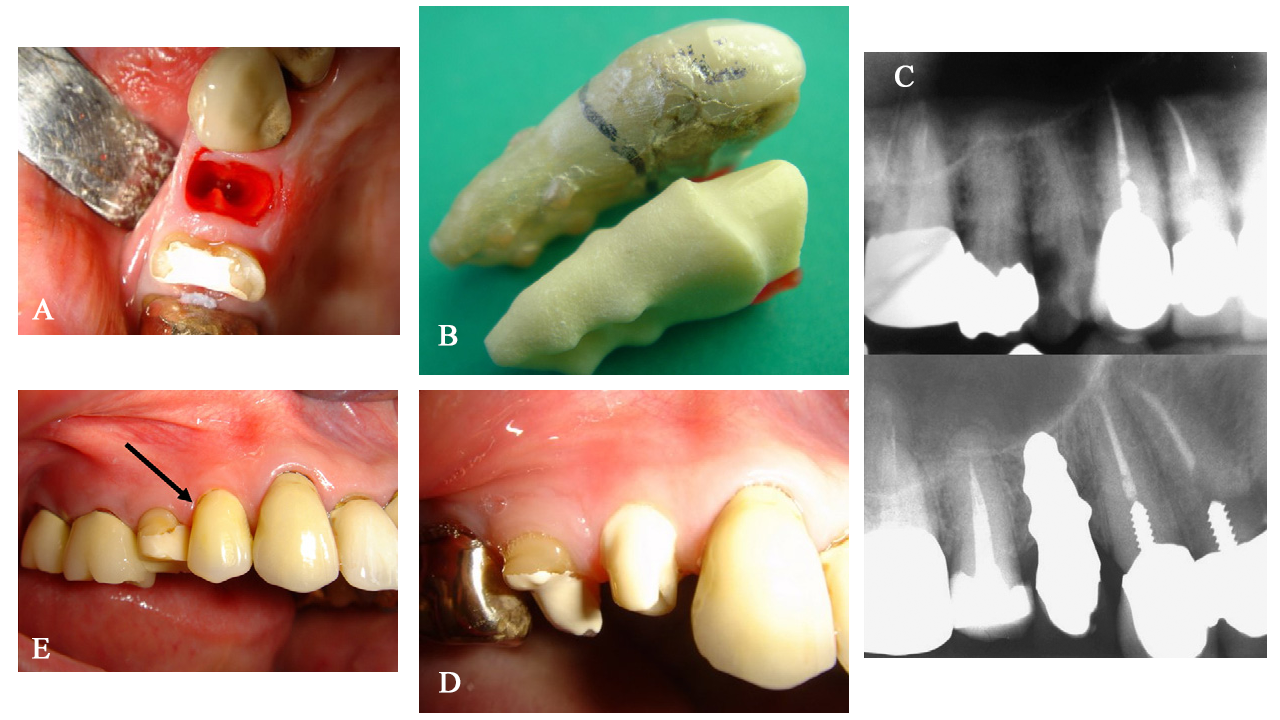
\includegraphics[width=0.9\textwidth,height=\textheight,keepaspectratio]{bioimplant}
    \caption{\textbf{\textit{Zirconia Root Analog Implant}}. \textbf{A}: Intact alveolus of a maxillary premolar. \textbf{B}: Premolar modified with composite retention near zirconia RAI. \textbf{C}: Pre-treatment (on top) and post-treatment radiography, after RAI insertion (at the bottom). \textbf{D}: RAI in place. \textbf{E}: 2 yearf after implant placement; healthy parodontal tissue with no sign of gingival retraction. From \emph{Pirker et al} \parencite{Reference86}}
    \label{fig:bioimplant}
    \end{center}
\vspace{-10pt}
\end{figure}

The same author then made a comparison between different topographies of zirconia RAI made with CAD-CAM technology in two group of patients \parencite{Reference87}. A group of patients was rehabilitated with RAI characterized by a rough surface created by sandblasting, while the second group was treated with sandblasted RAI on which macroretentions on the interdental surfaces were present. The group of sandblasted implants showed a success rate of 0\%, with all 6 implants inserted that failed before the application of the final crown. The group treated with macro-retention RAI showed a success rate of 92\% at two years, with only one implant lost on 12 inserted. The failure of the sandblasted implants was attributed to the uniform pressure exerted by the implant on the alveolus walls, instead in case of RAI with interproximal macroretention the distribution of the load in defined areas allowed to reduce the stress on the bone, favoring the osseointegration of the RAI. \\
Patankar \parencite{Reference88} replicated the zirconia RAI with interdental macroretentions of Pirker for the rehabilitation of a lower premolar, with a positive result.

\begin{wrapfigure} {R} {0.4\textwidth}
\vspace{-20pt}
	\begin{center}
	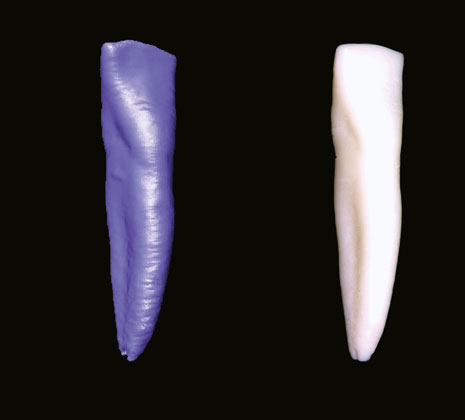
\includegraphics[width=0.4\textwidth, height=\textheight,keepaspectratio]{moin_dlp_zirconia}
    \caption{\textbf{Left}: CAD model of the tooth. \textbf{Right} DLP printend zirconia tooth. From \emph{Moin et al} \parencite{Reference89}}
    \label{fig:moin_dlp_zirconia}
    \end{center}
\vspace{-20pt}
\end{wrapfigure}

Moin \parencite{Reference89} used the Digital Light Processing (DLP) additive manufacturing technique to realize a zirconia replica of a dental element \ref{fig:moin_dlp_zirconia}. The author then digitally compared the CAD model of the replica, the scan of the printed zirconia replica and the scan of the original tooth, noting the adequate precision of the DLP technology for the additive manufacturing of zirconia products.\\
The production of ceramic objects is currently also possible using the extrusion printing technique, as documented by Nötzel \parencite{Reference97}. The process used by Nötzel consists in the production of a filament composed of paraffin, LDPE and Al2O3 particles; the filament is molded by extrusion to form the object, which is then subjected to chemical and thermal treatment for the removal of the medium in which the Al2O3 particles are dispersed, and finally sintered to give the final product. The extrusion printing of ceramic products is still to be evaluated in the manufacturing of dental products. \\

These reports show us that, using digital techniques, the production of Root Analog Implants is now possible in a precise manner and with the use of biomaterials that promote osteointegration and aesthetic and functional rehabilitation.\\
The correct evaluation of the alveolus and RAI morphology, and of the distribution of the masticatory forces on the alveolar bone is important in this perspective. The atraumatic avulsion of the tooth is at the basis of rehabilitation with RAI, because any trauma to the alveolus results in bone resorption and gingival retractions, with consequent degradation of the aesthetic characteristics of the prosthetic rehabilitation. The distribution of the forces on the alveolus walls is also to be precisely assessed. \\ With the RAI we seek primary stability by means of the dimensional congruity between the alveolus and the Rot Analog; it has been shown that excessive stress on the alveolus walls causes implant failure, probably due to reduction of the blood supply to the implant site and to the surrounding bone, which undergoes resorption. Further studies are necessary to asses the safety and standardization of the procedures here presented, but the anatomical implants could allow, in selected cases, a functional and aesthetic solution to the patient problem, and facilitate the resolution of post-extractive implants treatments maintaining high aesthetic standards.


\subsection{Prosthesis}
Rapid prototyping has been used both in fixed and removable prostheses, for the realization temporary restorations, aesthetic guides and mockups. Various additive manufacturing technologies and various materials have been used. \\
Tahayeri \parencite{Reference98} tested various features of SLA printing with specific dental resins (NextDent); he evalued the influence of some printing parameters on printing precision, mechanical properties and degree of conversion of the resin. The printed specimens proved to be in the precision range required for clinical use, as were the mechanical properties of the samples themselves. The author showed differences in the printing properties between various dental resins made by the same manufacturer, as well as different intensities of the printer's laser during the polymerization of the resins, depending on the darkness of the resins color and the relative light absorption rate. A selection of resins and printers optimized for combined use could further improve print accuracy; better results may be obtained from the fine adjustment of the printing parameters. \\
To be considered that, according to the manufacturer's indications, the resin would have had to undergo a second polymerization step after printing, which the authors did not perform to accelerate the eventual production process of the temporary restoration. Nevertheless, the mechanical properties of the non-post-polymerized resin have proved to be adequate to resist intraoral loads. \\
Katreva \parencite{Reference99} realized a workflow that integrate the use of 3D printed working models, the 3D printing of the temporary restoration and the printing of the final prosthesis for the pressed ceramic conversion. \\
Revilla-León \parencite{Reference100} used a digital workflow for the scanning of impressions, the creation of the diagnostic wax-up, the printing of a guide for the realization of the temporary restoration and finally for the production of the veneers, useful for aesthetic and functional rehabilitation of anterior sector of the maxillary arch. The guide for the construction of the provisionals was made using the DLP 3D printing technique, while the final lithium disilicate veneers were CAD-CAM milled. \\
Alharbi \parencite{Reference101} evaluated the possibility of making prosthetic crowns with SLA printing technique. The author measured the accuracy of the printed crown at various angles with respect to the horizontal plane and with the use of different size of supports. The same research group then evaluated the crown printing accuracy using the DLP \parencite{Reference102} printing technique. Both technologies proved to be accurate, with SLA printing which showed greater accuracy in replicating the morphology of the digital model. Both technologies are interesting for use in dentistry, but it is necessary to carry out further studies on the influence of the printing parameters on the final model and better explore the properties of the dental resins.
\begin{wrapfigure} {R} {0.4\textwidth}
\vspace{-20pt}
	\begin{center}
	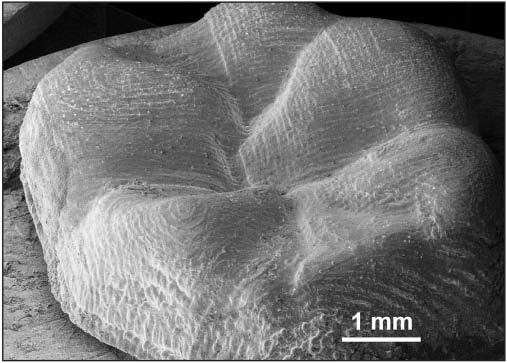
\includegraphics[width=0.4\textwidth, height=\textheight,keepaspectratio]{zircon_crown}
    \caption{Ink-jet 3D printed zirconia crown. From \emph{Ebert et al} \parencite{Reference106}}
    \label{fig:zircon_crown}
    \end{center}
\vspace{-20pt}
\end{wrapfigure}

Ebert printed zirconia crowns with a custom printer using the ink-jet technique. To make the crown, a zirconia-containing solution was deposited layer by layer to form the product, which was then sintered \ref{fig:zircon_crown}. This study has shown that zirconia crowns with good mechanical properties and precision for clinical use can be achieved by means of an additive ink-jet manufacturing process \parencite{Reference106}. \\
Alharbi \parencite{Reference107} evaluated the use of additive manufacturing in prosthetics, analyzing various reports and studies focusing on the fixed prosthesis and the partial and total removable prosthesis. The author has reported that the metal framework realized with the SLS (\emph{Selective Laser Sintering}) method are equivalent or more precise than the classical melting procedures, with respect to the gap between the metal framework and the dental abutment; in the same way the mechanical properties of the SLS products were equivalent or better than those realized with the classical procedures. Metal framework for the creation of removable partial dentures were produced by means of additive manufacturing either directly or indirectly. Direct manufacturing consists in printing the design by means of SLS processes; Indirect manufacturing consists in the realization of the castable resin product by means of SLA or DLP printing, the integration of the calcinable model in refractory material and the subsequent casting of the metal or alloy for the realization of the metallic framework. Both techniques for building removable prosthesis frameworks have shown acceptable accuracy, although the results are primarily derived from in vitro and case report studies. \\
Lin \parencite{Reference108} demonstrated a technique for the realization of provisional total prostheses through a digital protocol that provides optical scanning, digital diagnostic waxing of the prosthesis, printing of the prosthetic base and respective dental arch in separate phases, with resins of color and suitable characteristics; finally the union of arch and prosthetic base is achieved \ref{fig:separ_full_prot}. The study has not tested its use on the patient and there are no further reports of the clinical performance of total provisional removable prostheses made with this procedure and these materials. This concept could be explored, evaluating the accuracy compared to the other available manufacturing methods and the duration of the prosthesis over time, both from the perspective of the color and wear of the resin.\\
The available data on digital treatment planning techniques and the use of additive manufacturing technologies show promising prospects in dentistry, both for the production of temporaries \parencite{Reference125} and of removable prostheses \parencite{Reference107}. Further studies and evaluations with longer follow-up are still necessary before extensive clinical application of the technology. Furthermore, the possibility of producing definitive ceramic or zirconia prostheses, theoretically achievable with technologies such as SLS or inkjet printing, remains unexplored.
\begin{figure}[h]
\vspace{-10pt}
	\begin{center}
	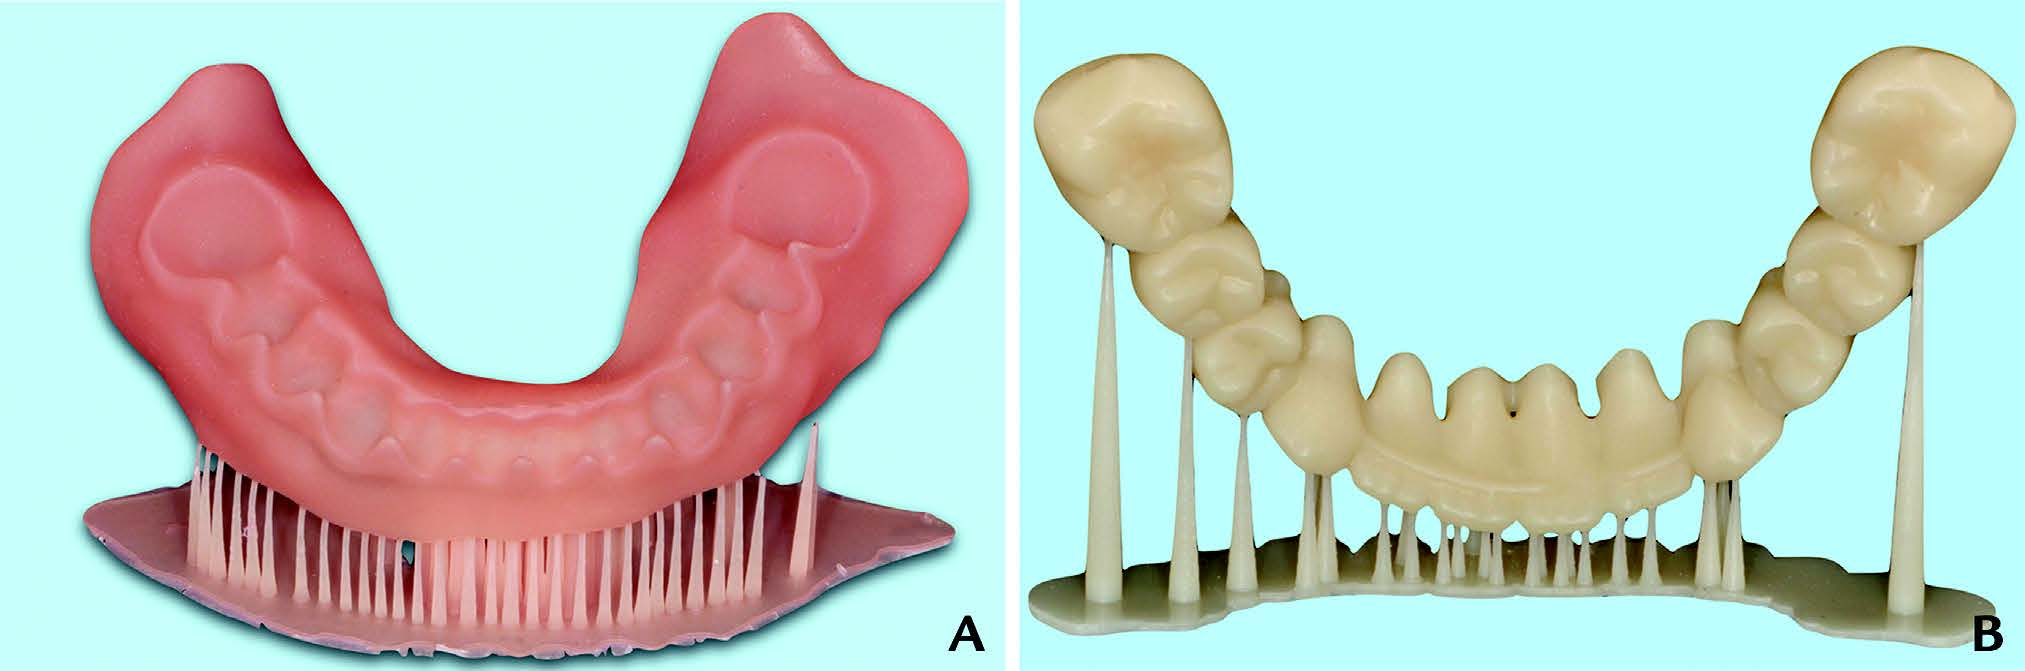
\includegraphics[width=0.9\textwidth,height=\textheight,keepaspectratio]{separ_full_prot}
    \caption{DLP printed removable prostesis. From \emph{Lin et al} \parencite{Reference108}}
    \label{fig:separ_full_prot}
    \end{center}
\vspace{-30pt}
\end{figure}

QUIQUIQUIRDTUYVOTDBIYDYR VSVUTSD

\subsection{Ortodonzia}
Orthodontics is one of the branches of dentistry that can best avail itself of the new possibilities of digital programming of treatment and the use of additive manufacturing technologies. Orthodontic therapy is classically programmed by means of teleradiographs, plaster models in the articulator and set of photos of the patient, in addition to the fundamental clinical and functional evaluation. The complex relationships between the bones of the skull involved in the oral function are difficult to analyze adequately on two-dimensional radiographs and with plaster models, especially if the treatment involves a surgical phase.\\
Digital orthodontic therapy can use the ability to print custom brackets \parencite{Reference115} and surgical guides for the insertion of orthodontic implants \parencite{Reference116} \ref{fig:stent_miniscrew}. 3D printing also facilitates the production of guides for positioning brackets in the patient \parencite{Reference127}, which favor a fast and precise positioning of the same, and of personalized auxiliary tools \parencite{Reference126}. The custom brackets were made by Krey through FreeCAD software and a DLP printing process \ref{fig:design_brackt}. With the same technique a positioning splint was printed, previously designed virtually, which allowed to position the brackets quickly and precisely. Intraoral scans at time intervals were performed and compared in MeshLab to verify the orthodontic movement of the dental elements; the post treatment retention splint was also virtually designed and printed in 3D. \\

\begin{figure}[h!]
\begin{subfigure}{0.5\textwidth}
\centering
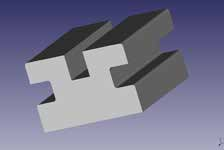
\includegraphics[width=0.9\linewidth, keepaspectratio]{design_brackt} 
\caption{Design CAD del bracket.}
\label{fig:design_brackt}
\end{subfigure}
\begin{subfigure}{0.5\textwidth}
\centering
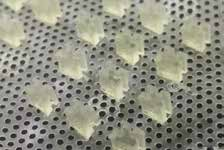
\includegraphics[width=0.9\linewidth, keepaspectratio]{printd_brackt}
\caption{Brackets stampati.}
\label{fig:printd_brackt}
\end{subfigure}
\begin{subfigure}{0.5\textwidth}
\centering
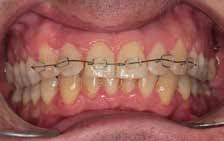
\includegraphics[width=0.9\linewidth, keepaspectratio]{working_brackt}
\caption{Brackets stampati in funzione all'interno del cavo orale.}
\label{fig:working_brackt}
\end{subfigure}
\begin{subfigure}{0.5\textwidth}
\centering
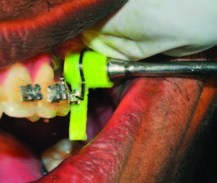
\includegraphics[width=0.7\linewidth, keepaspectratio]{stent_miniscrew}
\caption{Guida per l'inserimento di impianti ortodontici stampata in 3D}
\label{fig:stent_miniscrew}
\end{subfigure}
\caption{A, B e C da \emph{Krey et al} \parencite{Reference115}, D da \emph{Ahamed et al} \parencite{Reference116}}
\label{fig:3d_ortho}
\end{figure}

This was a test study with brackets \emph{edgewise} molded in light-curable resin; the authors suggested the possibility of revising part of the design to optimize the resistance of the brackets. The report is generally positive and opens up the possibility of a radical change in the way in which orthodontics with fixed devices can be performed in the dental office, with the transition from the use of generic brackets to custom brackets achievable in the clinic.
In modern dental practice, the use of plaster models is often accompanied by digital scans and 3D printing of the model. Several authors have evaluated the accuracy of models made with additive manufacturing techniques, with different results. Dietrich \parencite{Reference112} evaluated the accuracy and accuracy of dental models made with polyjet and SLA techniques. The printed models were scanned and evaluated via software to evaluate the discrepancy with the original. Both methods of printing proved to be capable of printing accuracy suitable for orthodontic use, with a maximum detected error of about \SI{100}{\micro\metre}. \\
Wan Hassan \parencite{Reference113} manually compared, by means of a caliber, dental arched models of patients, made of plaster and printed with SLA technology. The author has decreed the models not suitable for orthodontic use due to a discrepancy of about 1mm compared to the original. The author reports that the digital scanning of the plaster models resulted in a loss of detail, moreover the measurements with gauge were sometimes not easy to carry out due to the overcrowding. Both of these conditions may have contributed to the reported error. Removable devices can also be manufactured with 3D printing \parencite{Reference111}. In addition, 3D printed surgical guides have been used to perform cortical osteotomies in order to accelerate orthodontic movements \parencite{Reference114}. \\
The possibility of integration that digital orthodontics also allows us from the biomechanical point of view is very important. The use of optical scans and CBCT allows detailed information on the patient's structure. Orthodontic movements are based on biological and physical principles, where controlled forces are used to activate the bone remodeling process, which allows the movement of the dental element. These factors could be investigated by integrating the anatomical data (bones, muscles, ligaments, organs) and functional data (masticatory force, mechanical characteristics of the tissues and materials involved, range of mandibular movement \ldots) to simulate in silico treatment, providing to the patient a personalized treatment according to its biological and response characteristics \parencite{Reference110}, \parencite{Reference140}.
\begin{figure}[h]
\vspace{-10pt}
	\begin{center}
	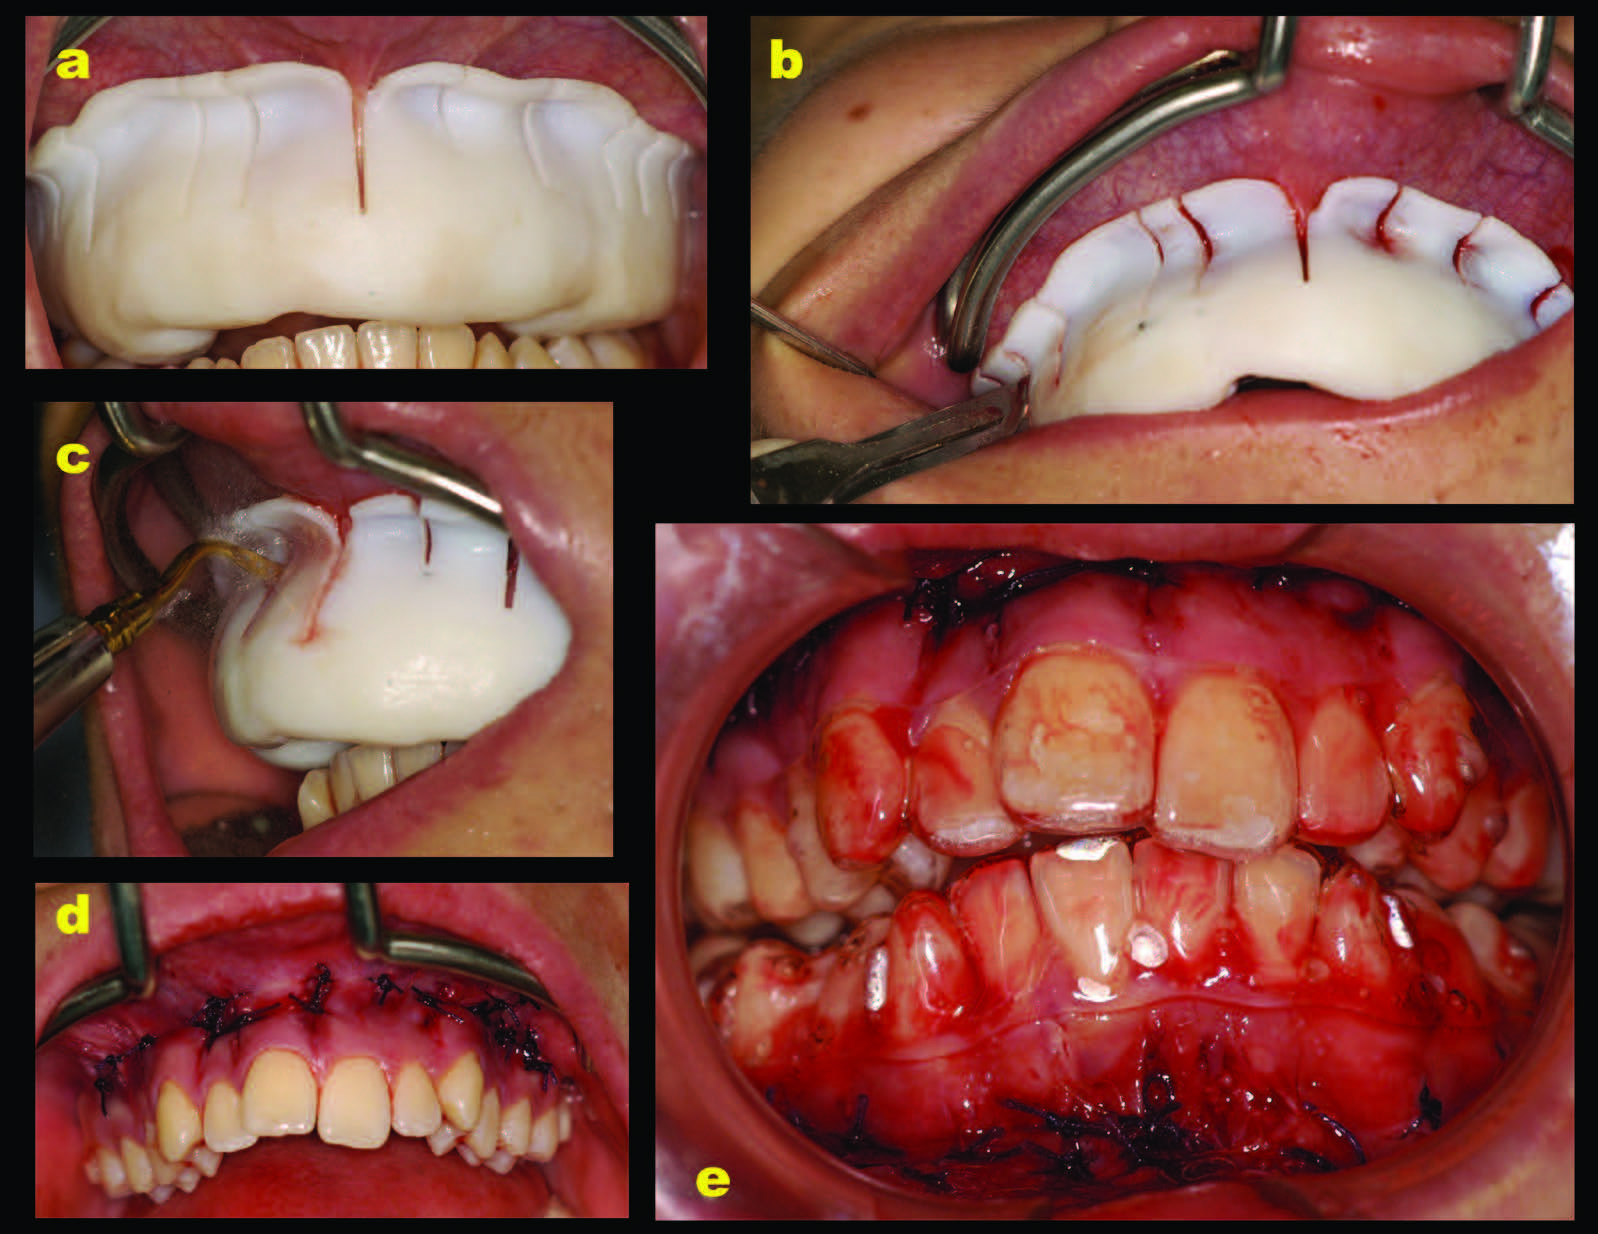
\includegraphics[width=0.9\textwidth, keepaspectratio]{guide}
    \caption{Posizionamento della guida chirurgica stampata in 3D per l'esecuzione di osteotomie flapless. \textbf{a}: Valutazione della stabilità intraorale. \textbf{b}: incisioni verticali della gengiva con bisturi n15. \textbf{c}: corticotomie verticali eseguite usando uno strumento piezoelettrico. \textbf{d}: sutura delle incisioni. \textbf{e}: posizionamento degli allineatori trasparenti dopo la chirurgia. Da \emph{Cassetta et al} \parencite{Reference114}.}
    \label{fig:guide}
	\end{center}
\vspace{-20pt}
\end{figure}

 
 